% !TEX TS-program = pdflatex
% !TEX encoding = UTF-8 Unicode
\documentclass[border=0mm]{standalone}
% packages
\usepackage{tikz}
\usetikzlibrary{patterns}
\usepackage{amsmath,amssymb}
\usepackage{bm}
\usepackage{pgfplots}
\pgfplotsset{compat=1.15}
% start document
\begin{document}
% generated by ROOT (CERN)
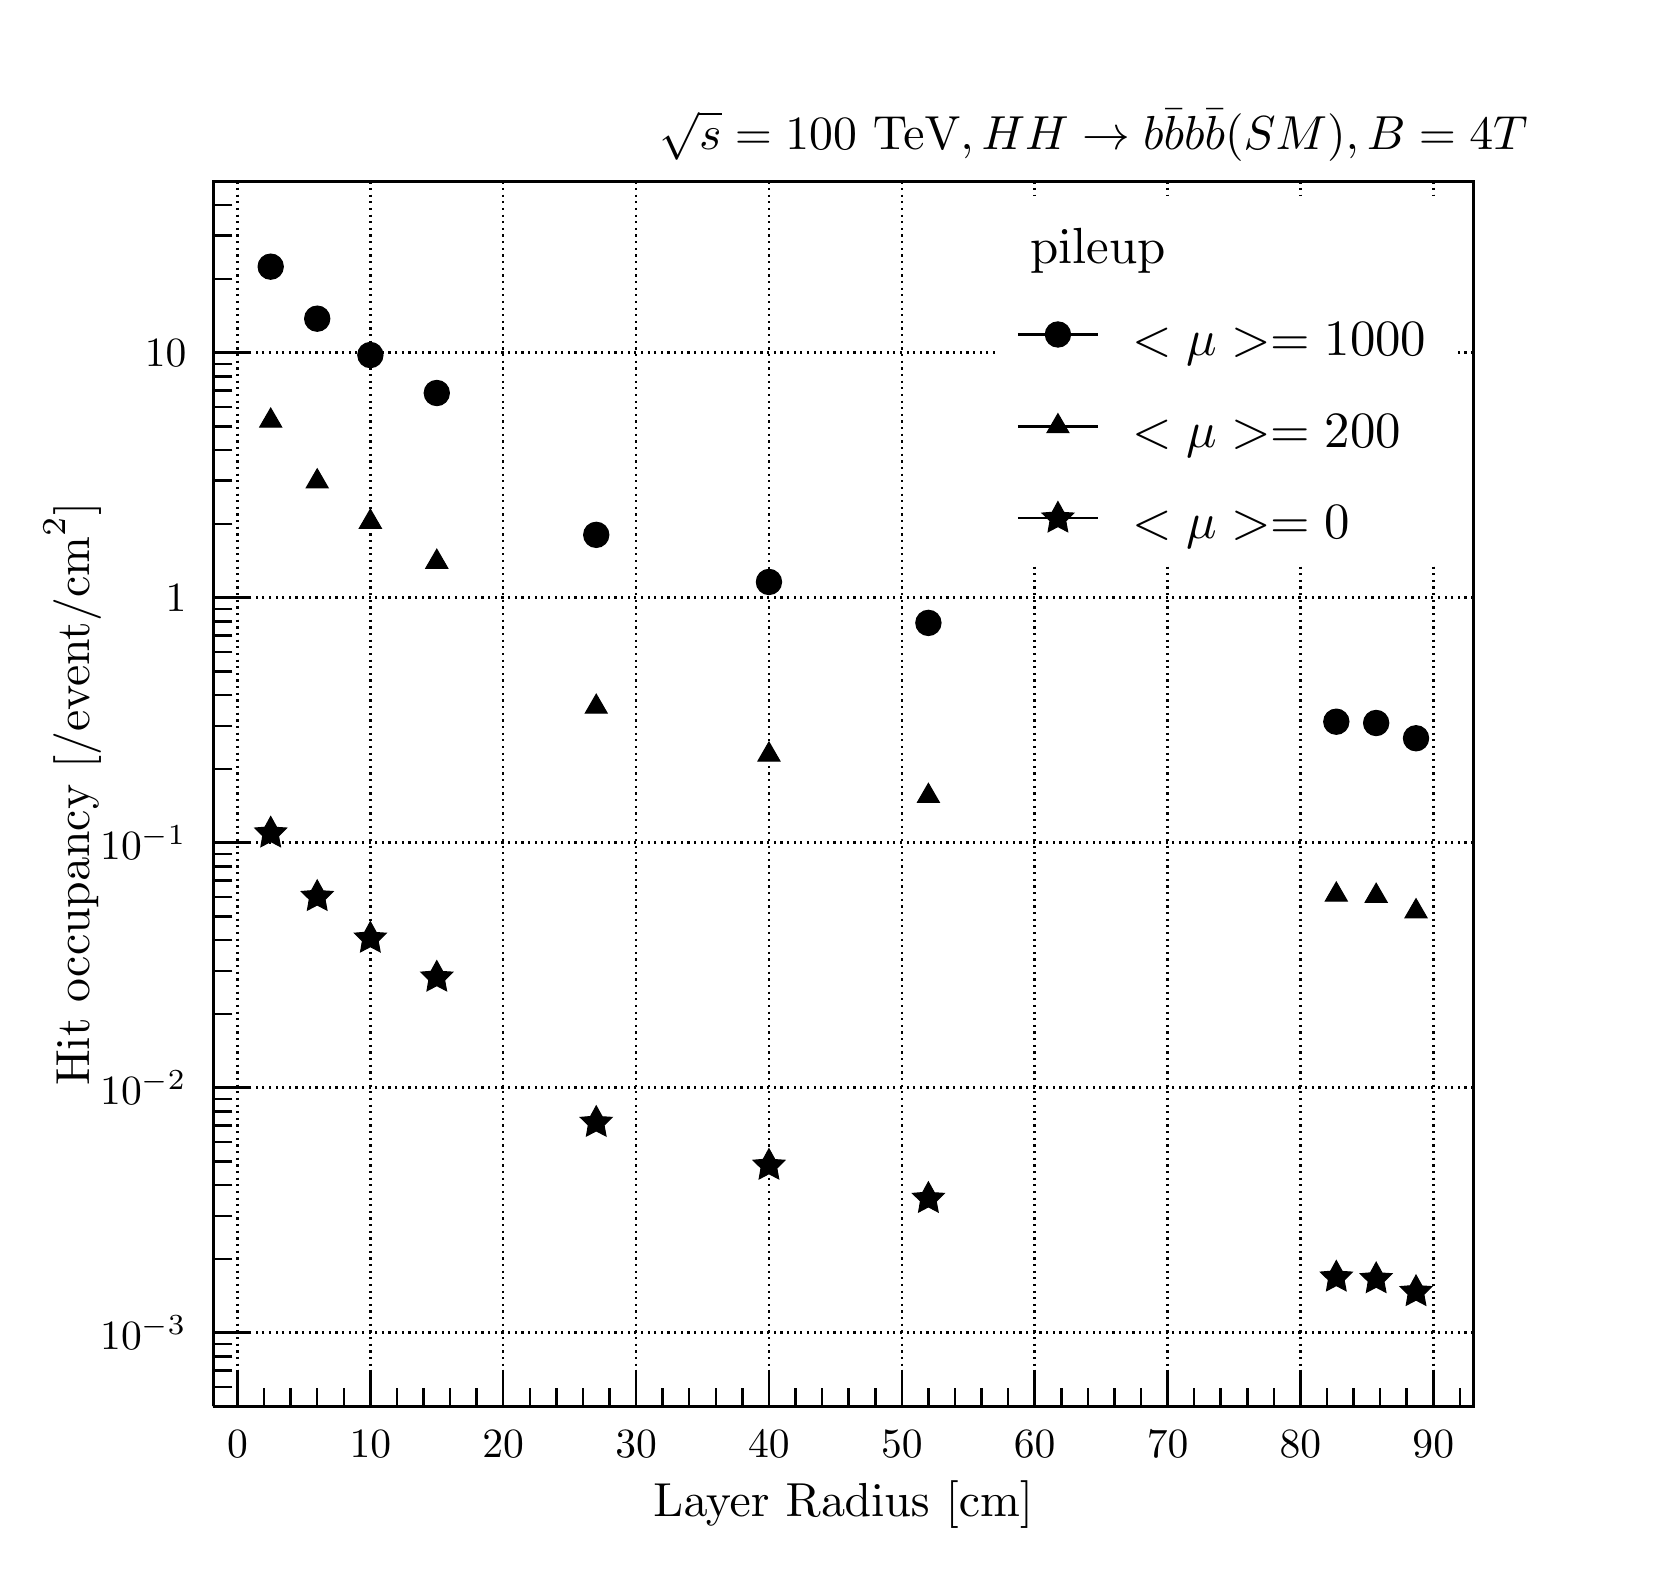
\begin{tikzpicture}
\pgfdeclareplotmark{cross} {
\pgfpathmoveto{\pgfpoint{-0.3\pgfplotmarksize}{\pgfplotmarksize}}
\pgfpathlineto{\pgfpoint{+0.3\pgfplotmarksize}{\pgfplotmarksize}}
\pgfpathlineto{\pgfpoint{+0.3\pgfplotmarksize}{0.3\pgfplotmarksize}}
\pgfpathlineto{\pgfpoint{+1\pgfplotmarksize}{0.3\pgfplotmarksize}}
\pgfpathlineto{\pgfpoint{+1\pgfplotmarksize}{-0.3\pgfplotmarksize}}
\pgfpathlineto{\pgfpoint{+0.3\pgfplotmarksize}{-0.3\pgfplotmarksize}}
\pgfpathlineto{\pgfpoint{+0.3\pgfplotmarksize}{-1.\pgfplotmarksize}}
\pgfpathlineto{\pgfpoint{-0.3\pgfplotmarksize}{-1.\pgfplotmarksize}}
\pgfpathlineto{\pgfpoint{-0.3\pgfplotmarksize}{-0.3\pgfplotmarksize}}
\pgfpathlineto{\pgfpoint{-1.\pgfplotmarksize}{-0.3\pgfplotmarksize}}
\pgfpathlineto{\pgfpoint{-1.\pgfplotmarksize}{0.3\pgfplotmarksize}}
\pgfpathlineto{\pgfpoint{-0.3\pgfplotmarksize}{0.3\pgfplotmarksize}}
\pgfpathclose
\pgfusepathqstroke
}
\pgfdeclareplotmark{cross*} {
\pgfpathmoveto{\pgfpoint{-0.3\pgfplotmarksize}{\pgfplotmarksize}}
\pgfpathlineto{\pgfpoint{+0.3\pgfplotmarksize}{\pgfplotmarksize}}
\pgfpathlineto{\pgfpoint{+0.3\pgfplotmarksize}{0.3\pgfplotmarksize}}
\pgfpathlineto{\pgfpoint{+1\pgfplotmarksize}{0.3\pgfplotmarksize}}
\pgfpathlineto{\pgfpoint{+1\pgfplotmarksize}{-0.3\pgfplotmarksize}}
\pgfpathlineto{\pgfpoint{+0.3\pgfplotmarksize}{-0.3\pgfplotmarksize}}
\pgfpathlineto{\pgfpoint{+0.3\pgfplotmarksize}{-1.\pgfplotmarksize}}
\pgfpathlineto{\pgfpoint{-0.3\pgfplotmarksize}{-1.\pgfplotmarksize}}
\pgfpathlineto{\pgfpoint{-0.3\pgfplotmarksize}{-0.3\pgfplotmarksize}}
\pgfpathlineto{\pgfpoint{-1.\pgfplotmarksize}{-0.3\pgfplotmarksize}}
\pgfpathlineto{\pgfpoint{-1.\pgfplotmarksize}{0.3\pgfplotmarksize}}
\pgfpathlineto{\pgfpoint{-0.3\pgfplotmarksize}{0.3\pgfplotmarksize}}
\pgfpathclose
\pgfusepathqfillstroke
}
\pgfdeclareplotmark{newstar} {
\pgfpathmoveto{\pgfqpoint{0pt}{\pgfplotmarksize}}
\pgfpathlineto{\pgfqpointpolar{44}{0.5\pgfplotmarksize}}
\pgfpathlineto{\pgfqpointpolar{18}{\pgfplotmarksize}}
\pgfpathlineto{\pgfqpointpolar{-20}{0.5\pgfplotmarksize}}
\pgfpathlineto{\pgfqpointpolar{-54}{\pgfplotmarksize}}
\pgfpathlineto{\pgfqpointpolar{-90}{0.5\pgfplotmarksize}}
\pgfpathlineto{\pgfqpointpolar{234}{\pgfplotmarksize}}
\pgfpathlineto{\pgfqpointpolar{198}{0.5\pgfplotmarksize}}
\pgfpathlineto{\pgfqpointpolar{162}{\pgfplotmarksize}}
\pgfpathlineto{\pgfqpointpolar{134}{0.5\pgfplotmarksize}}
\pgfpathclose
\pgfusepathqstroke
}
\pgfdeclareplotmark{newstar*} {
\pgfpathmoveto{\pgfqpoint{0pt}{\pgfplotmarksize}}
\pgfpathlineto{\pgfqpointpolar{44}{0.5\pgfplotmarksize}}
\pgfpathlineto{\pgfqpointpolar{18}{\pgfplotmarksize}}
\pgfpathlineto{\pgfqpointpolar{-20}{0.5\pgfplotmarksize}}
\pgfpathlineto{\pgfqpointpolar{-54}{\pgfplotmarksize}}
\pgfpathlineto{\pgfqpointpolar{-90}{0.5\pgfplotmarksize}}
\pgfpathlineto{\pgfqpointpolar{234}{\pgfplotmarksize}}
\pgfpathlineto{\pgfqpointpolar{198}{0.5\pgfplotmarksize}}
\pgfpathlineto{\pgfqpointpolar{162}{\pgfplotmarksize}}
\pgfpathlineto{\pgfqpointpolar{134}{0.5\pgfplotmarksize}}
\pgfpathclose
\pgfusepathqfillstroke
}
\definecolor{c}{rgb}{1,1,1};
\draw [color=c, fill=c] (0,0) rectangle (20,19.4486);
\draw [color=c, fill=c] (2,1.94486) rectangle (18,17.5038);
\definecolor{c}{rgb}{0,0,0};
\draw [c,line width=0.9] (2,1.94486) -- (2,17.5038) -- (18,17.5038) -- (18,1.94486) -- (2,1.94486);
\definecolor{c}{rgb}{1,1,1};
\draw [color=c, fill=c] (2,1.94486) rectangle (18,17.5038);
\definecolor{c}{rgb}{0,0,0};
\draw [c,line width=0.9] (2,1.94486) -- (2,17.5038) -- (18,17.5038) -- (18,1.94486) -- (2,1.94486);
\draw [c,line width=0.9] (2,1.94486) -- (18,1.94486);
\draw [c,dash pattern=on 0.80pt off 1.60pt ,line width=0.9] (2.30542,17.5038) -- (2.30542,1.94486);
\draw [c,dash pattern=on 0.80pt off 1.60pt ,line width=0.9] (3.99283,17.5038) -- (3.99283,1.94486);
\draw [c,dash pattern=on 0.80pt off 1.60pt ,line width=0.9] (5.68024,17.5038) -- (5.68024,1.94486);
\draw [c,dash pattern=on 0.80pt off 1.60pt ,line width=0.9] (7.36764,17.5038) -- (7.36764,1.94486);
\draw [c,dash pattern=on 0.80pt off 1.60pt ,line width=0.9] (9.05505,17.5038) -- (9.05505,1.94486);
\draw [c,dash pattern=on 0.80pt off 1.60pt ,line width=0.9] (10.7425,17.5038) -- (10.7425,1.94486);
\draw [c,dash pattern=on 0.80pt off 1.60pt ,line width=0.9] (12.4299,17.5038) -- (12.4299,1.94486);
\draw [c,dash pattern=on 0.80pt off 1.60pt ,line width=0.9] (14.1173,17.5038) -- (14.1173,1.94486);
\draw [c,dash pattern=on 0.80pt off 1.60pt ,line width=0.9] (15.8047,17.5038) -- (15.8047,1.94486);
\draw [c,dash pattern=on 0.80pt off 1.60pt ,line width=0.9] (17.4921,17.5038) -- (17.4921,1.94486);
\draw [c,dash pattern=on 0.80pt off 1.60pt ,line width=0.9] (2.30542,17.5038) -- (2.30542,1.94486);
\draw [c,dash pattern=on 0.80pt off 1.60pt ,line width=0.9] (17.4921,17.5038) -- (17.4921,1.94486);
\draw [c,line width=0.9] (2,1.94486) -- (2,17.5038);
\draw [c,dash pattern=on 0.80pt off 1.60pt ,line width=0.9] (18,2.8816) -- (2,2.8816);
\draw [c,dash pattern=on 0.80pt off 1.60pt ,line width=0.9] (18,5.99338) -- (2,5.99338);
\draw [c,dash pattern=on 0.80pt off 1.60pt ,line width=0.9] (18,9.10516) -- (2,9.10516);
\draw [c,dash pattern=on 0.80pt off 1.60pt ,line width=0.9] (18,12.2169) -- (2,12.2169);
\draw [c,dash pattern=on 0.80pt off 1.60pt ,line width=0.9] (18,15.3287) -- (2,15.3287);
\draw [c,line width=0.9] (2,1.94486) -- (18,1.94486);
\draw [c,line width=0.9] (2.30542,2.41163) -- (2.30542,1.94486);
\draw [c,line width=0.9] (2.6429,2.17825) -- (2.6429,1.94486);
\draw [c,line width=0.9] (2.98038,2.17825) -- (2.98038,1.94486);
\draw [c,line width=0.9] (3.31787,2.17825) -- (3.31787,1.94486);
\draw [c,line width=0.9] (3.65535,2.17825) -- (3.65535,1.94486);
\draw [c,line width=0.9] (3.99283,2.41163) -- (3.99283,1.94486);
\draw [c,line width=0.9] (4.33031,2.17825) -- (4.33031,1.94486);
\draw [c,line width=0.9] (4.66779,2.17825) -- (4.66779,1.94486);
\draw [c,line width=0.9] (5.00527,2.17825) -- (5.00527,1.94486);
\draw [c,line width=0.9] (5.34275,2.17825) -- (5.34275,1.94486);
\draw [c,line width=0.9] (5.68024,2.41163) -- (5.68024,1.94486);
\draw [c,line width=0.9] (6.01772,2.17825) -- (6.01772,1.94486);
\draw [c,line width=0.9] (6.3552,2.17825) -- (6.3552,1.94486);
\draw [c,line width=0.9] (6.69268,2.17825) -- (6.69268,1.94486);
\draw [c,line width=0.9] (7.03016,2.17825) -- (7.03016,1.94486);
\draw [c,line width=0.9] (7.36764,2.41163) -- (7.36764,1.94486);
\draw [c,line width=0.9] (7.70513,2.17825) -- (7.70513,1.94486);
\draw [c,line width=0.9] (8.04261,2.17825) -- (8.04261,1.94486);
\draw [c,line width=0.9] (8.38009,2.17825) -- (8.38009,1.94486);
\draw [c,line width=0.9] (8.71757,2.17825) -- (8.71757,1.94486);
\draw [c,line width=0.9] (9.05505,2.41163) -- (9.05505,1.94486);
\draw [c,line width=0.9] (9.39253,2.17825) -- (9.39253,1.94486);
\draw [c,line width=0.9] (9.73001,2.17825) -- (9.73001,1.94486);
\draw [c,line width=0.9] (10.0675,2.17825) -- (10.0675,1.94486);
\draw [c,line width=0.9] (10.405,2.17825) -- (10.405,1.94486);
\draw [c,line width=0.9] (10.7425,2.41163) -- (10.7425,1.94486);
\draw [c,line width=0.9] (11.0799,2.17825) -- (11.0799,1.94486);
\draw [c,line width=0.9] (11.4174,2.17825) -- (11.4174,1.94486);
\draw [c,line width=0.9] (11.7549,2.17825) -- (11.7549,1.94486);
\draw [c,line width=0.9] (12.0924,2.17825) -- (12.0924,1.94486);
\draw [c,line width=0.9] (12.4299,2.41163) -- (12.4299,1.94486);
\draw [c,line width=0.9] (12.7673,2.17825) -- (12.7673,1.94486);
\draw [c,line width=0.9] (13.1048,2.17825) -- (13.1048,1.94486);
\draw [c,line width=0.9] (13.4423,2.17825) -- (13.4423,1.94486);
\draw [c,line width=0.9] (13.7798,2.17825) -- (13.7798,1.94486);
\draw [c,line width=0.9] (14.1173,2.41163) -- (14.1173,1.94486);
\draw [c,line width=0.9] (14.4548,2.17825) -- (14.4548,1.94486);
\draw [c,line width=0.9] (14.7922,2.17825) -- (14.7922,1.94486);
\draw [c,line width=0.9] (15.1297,2.17825) -- (15.1297,1.94486);
\draw [c,line width=0.9] (15.4672,2.17825) -- (15.4672,1.94486);
\draw [c,line width=0.9] (15.8047,2.41163) -- (15.8047,1.94486);
\draw [c,line width=0.9] (16.1422,2.17825) -- (16.1422,1.94486);
\draw [c,line width=0.9] (16.4796,2.17825) -- (16.4796,1.94486);
\draw [c,line width=0.9] (16.8171,2.17825) -- (16.8171,1.94486);
\draw [c,line width=0.9] (17.1546,2.17825) -- (17.1546,1.94486);
\draw [c,line width=0.9] (17.4921,2.41163) -- (17.4921,1.94486);
\draw [c,line width=0.9] (2.30542,2.41163) -- (2.30542,1.94486);
\draw [c,line width=0.9] (17.4921,2.41163) -- (17.4921,1.94486);
\draw [c,line width=0.9] (17.8296,2.17825) -- (17.8296,1.94486);
\draw [anchor=base] (2.30542,1.30306) node[scale=1.50291, color=c, rotate=0]{0};
\draw [anchor=base] (3.99283,1.30306) node[scale=1.50291, color=c, rotate=0]{10};
\draw [anchor=base] (5.68024,1.30306) node[scale=1.50291, color=c, rotate=0]{20};
\draw [anchor=base] (7.36764,1.30306) node[scale=1.50291, color=c, rotate=0]{30};
\draw [anchor=base] (9.05505,1.30306) node[scale=1.50291, color=c, rotate=0]{40};
\draw [anchor=base] (10.7425,1.30306) node[scale=1.50291, color=c, rotate=0]{50};
\draw [anchor=base] (12.4299,1.30306) node[scale=1.50291, color=c, rotate=0]{60};
\draw [anchor=base] (14.1173,1.30306) node[scale=1.50291, color=c, rotate=0]{70};
\draw [anchor=base] (15.8047,1.30306) node[scale=1.50291, color=c, rotate=0]{80};
\draw [anchor=base] (17.4921,1.30306) node[scale=1.50291, color=c, rotate=0]{90};
\draw (10,0.700151) node[scale=1.72557, color=c, rotate=0]{Layer Radius [cm]};
\draw [c,line width=0.9] (2,1.94486) -- (2,17.5038);
\draw [c,line width=0.9] (2.24,1.94487) -- (2,1.94487);
\draw [c,line width=0.9] (2.24,2.19126) -- (2,2.19126);
\draw [c,line width=0.9] (2.24,2.39958) -- (2,2.39958);
\draw [c,line width=0.9] (2.24,2.58004) -- (2,2.58004);
\draw [c,line width=0.9] (2.24,2.73922) -- (2,2.73922);
\draw [c,line width=0.9] (2.48,2.8816) -- (2,2.8816);
\draw [anchor= east] (1.844,2.8816) node[scale=1.50291, color=c, rotate=0]{$10^{-3}$};
\draw [c,line width=0.9] (2.24,3.81834) -- (2,3.81834);
\draw [c,line width=0.9] (2.24,4.3663) -- (2,4.3663);
\draw [c,line width=0.9] (2.24,4.75508) -- (2,4.75508);
\draw [c,line width=0.9] (2.24,5.05664) -- (2,5.05664);
\draw [c,line width=0.9] (2.24,5.30304) -- (2,5.30304);
\draw [c,line width=0.9] (2.24,5.51136) -- (2,5.51136);
\draw [c,line width=0.9] (2.24,5.69182) -- (2,5.69182);
\draw [c,line width=0.9] (2.24,5.851) -- (2,5.851);
\draw [c,line width=0.9] (2.48,5.99338) -- (2,5.99338);
\draw [anchor= east] (1.844,5.99338) node[scale=1.50291, color=c, rotate=0]{$10^{-2}$};
\draw [c,line width=0.9] (2.24,6.93012) -- (2,6.93012);
\draw [c,line width=0.9] (2.24,7.47808) -- (2,7.47808);
\draw [c,line width=0.9] (2.24,7.86686) -- (2,7.86686);
\draw [c,line width=0.9] (2.24,8.16842) -- (2,8.16842);
\draw [c,line width=0.9] (2.24,8.41482) -- (2,8.41482);
\draw [c,line width=0.9] (2.24,8.62314) -- (2,8.62314);
\draw [c,line width=0.9] (2.24,8.8036) -- (2,8.8036);
\draw [c,line width=0.9] (2.24,8.96277) -- (2,8.96277);
\draw [c,line width=0.9] (2.48,9.10516) -- (2,9.10516);
\draw [anchor= east] (1.844,9.10516) node[scale=1.50291, color=c, rotate=0]{$10^{-1}$};
\draw [c,line width=0.9] (2.24,10.0419) -- (2,10.0419);
\draw [c,line width=0.9] (2.24,10.5899) -- (2,10.5899);
\draw [c,line width=0.9] (2.24,10.9786) -- (2,10.9786);
\draw [c,line width=0.9] (2.24,11.2802) -- (2,11.2802);
\draw [c,line width=0.9] (2.24,11.5266) -- (2,11.5266);
\draw [c,line width=0.9] (2.24,11.7349) -- (2,11.7349);
\draw [c,line width=0.9] (2.24,11.9154) -- (2,11.9154);
\draw [c,line width=0.9] (2.24,12.0746) -- (2,12.0746);
\draw [c,line width=0.9] (2.48,12.2169) -- (2,12.2169);
\draw [anchor= east] (1.844,12.2169) node[scale=1.50291, color=c, rotate=0]{1};
\draw [c,line width=0.9] (2.24,13.1537) -- (2,13.1537);
\draw [c,line width=0.9] (2.24,13.7016) -- (2,13.7016);
\draw [c,line width=0.9] (2.24,14.0904) -- (2,14.0904);
\draw [c,line width=0.9] (2.24,14.392) -- (2,14.392);
\draw [c,line width=0.9] (2.24,14.6384) -- (2,14.6384);
\draw [c,line width=0.9] (2.24,14.8467) -- (2,14.8467);
\draw [c,line width=0.9] (2.24,15.0272) -- (2,15.0272);
\draw [c,line width=0.9] (2.24,15.1863) -- (2,15.1863);
\draw [c,line width=0.9] (2.48,15.3287) -- (2,15.3287);
\draw [anchor= east] (1.844,15.3287) node[scale=1.50291, color=c, rotate=0]{10};
\draw [c,line width=0.9] (2.24,16.2655) -- (2,16.2655);
\draw [c,line width=0.9] (2.24,16.8134) -- (2,16.8134);
\draw [c,line width=0.9] (2.24,17.2022) -- (2,17.2022);
\draw [c,line width=0.9] (2.24,17.5038) -- (2,17.5038);
\draw (0.208,9.72431) node[scale=1.72557, color=c, rotate=90]{$\text{Hit occupancy }[/\text{event/cm}^{2}]$};
\foreach \P in {(2.72727,16.4203), (3.31787,15.7598), (3.99283,15.2979), (4.83653,14.8157), (6.86142,13.0143), (9.05505,12.416), (11.0799,11.8961)}{\draw[mark options={color=c,fill=c},mark size=4.564565pt,mark=*] plot coordinates {\P};}
\foreach \P in {(16.2603,10.6413), (16.7665,10.6249), (17.2727,10.4311)}{\draw[mark options={color=c,fill=c},mark size=4.564565pt,mark=*] plot coordinates {\P};}
\foreach \P in {(2.72727,14.4633), (3.31787,13.6917), (3.99283,13.179), (4.83653,12.671), (6.86142,10.8296), (9.05505,10.2222), (11.0799,9.69694)}{\draw[mark options={color=c,fill=c},mark size=4.564565pt,mark=triangle*] plot coordinates {\P};}
\foreach \P in {(16.2603,8.44433), (16.7665,8.42861), (17.2727,8.23235)}{\draw[mark options={color=c,fill=c},mark size=4.564565pt,mark=triangle*] plot coordinates {\P};}
\foreach \P in {(2.72727,9.22544), (3.31787,8.41926), (3.99283,7.88989), (4.83653,7.39513), (6.86142,5.55064), (9.05505,5.00634), (11.0799,4.58551)}{\draw[mark options={color=c,fill=c},mark size=6.006006pt,mark=newstar*] plot coordinates {\P};}
\foreach \P in {(16.2603,3.58589), (16.7665,3.56548), (17.2727,3.40163)}{\draw[mark options={color=c,fill=c},mark size=6.006006pt,mark=newstar*] plot coordinates {\P};}
\draw [anchor= west] (7.45,18.0872) node[scale=1.72557, color=c, rotate=0]{$\sqrt{s} = 100 ~\text{TeV}, HH \rightarrow b\bar{b}b\bar{b}(SM), B=4T$};
\definecolor{c}{rgb}{1,1,1};
\draw [color=c, fill=c] (12,12.6416) rectangle (17.8,17.3093);
\definecolor{c}{rgb}{0,0,0};
%\draw [c,line width=0.9] (12,12.6416) -- (17.8,12.6416);
%\draw [c,line width=0.9] (17.8,12.6416) -- (17.8,17.3093);
%\draw [c,line width=0.9] (17.8,17.3093) -- (12,17.3093);
%\draw [c,line width=0.9] (12,17.3093) -- (12,12.6416);
\draw [anchor=base west] (12.145,16.4633) node[scale=1.83689, color=c, rotate=0]{pileup};
\draw [anchor=base west] (13.45,15.2963) node[scale=1.83689, color=c, rotate=0]{$<\mu> = 1000$};
\definecolor{c}{rgb}{1,1,1};
\draw [c] (12.2175,15.1505) -- (13.2325,15.1505) -- (13.2325,15.9673) -- (12.2175,15.9673);
\definecolor{c}{rgb}{0,0,0};
\draw [c,line width=0.9] (12.2175,15.5589) -- (13.2325,15.5589);
\foreach \P in {(12.725,15.5589)}{\draw[mark options={color=c,fill=c},mark size=4.564565pt,mark=*] plot coordinates {\P};}
\draw [anchor=base west] (13.45,14.1294) node[scale=1.83689, color=c, rotate=0]{$<\mu> = 200$};
\definecolor{c}{rgb}{1,1,1};
\draw [c] (12.2175,13.9836) -- (13.2325,13.9836) -- (13.2325,14.8004) -- (12.2175,14.8004);
\definecolor{c}{rgb}{0,0,0};
\draw [c,line width=0.9] (12.2175,14.392) -- (13.2325,14.392);
\foreach \P in {(12.725,14.392)}{\draw[mark options={color=c,fill=c},mark size=4.564565pt,mark=triangle*] plot coordinates {\P};}
\draw [anchor=base west] (13.45,12.9625) node[scale=1.83689, color=c, rotate=0]{$<\mu> = 0$};
\definecolor{c}{rgb}{1,1,1};
\draw [c] (12.2175,12.8166) -- (13.2325,12.8166) -- (13.2325,13.6335) -- (12.2175,13.6335);
\definecolor{c}{rgb}{0,0,0};
\draw [c,line width=0.9] (12.2175,13.2251) -- (13.2325,13.2251);
\foreach \P in {(12.725,13.2251)}{\draw[mark options={color=c,fill=c},mark size=6.006006pt,mark=newstar*] plot coordinates {\P};}
\end{tikzpicture}
% end document
\end{document}
